%%
% La siguiente plantilla esta basada en el siguiente enlace:
% http://academic.reed.edu/physics/courses/Physics332.s08/reports.html
% La plantilla original puede descargarse de ese sitio
% Se dejo parte del texto original en inglés para ilustar el uso de la plantilla
% Se hicieron algunas modificaciones para ajustar el idioma y otros detalles para 
% completar un reporte técnico breve pero muy puntual
% Modificación Inicial: Marco Aurelio Nuno Maganda - 11/SEP/2014
% 
% Enlace a la documentación del tipo de documento base (revtex4)
% http://mirror.hmc.edu/ctan/macros/latex/contrib/revtex/doc/latex/revtex/source/revtex4-1.pdf
%
% En algunas distribuciones es necesario instalar el paquete texlive-publishers
%
%\documentclass[letterpaper,aps,twocolumn,pre,nofootinbib]{revtex4}
%\documentclass[twocolumn]{article}
\documentclass[conference]{IEEEtran}
\usepackage[spanish]{babel}
\usepackage{amsmath,amssymb,amsfonts,amsthm}
\usepackage{graphicx}
%\usepackage{bbm}
\usepackage[utf8]{inputenc} % Caracteres en Español (Acentos, ñs)
\usepackage{url} % ACENTOS
\usepackage{hyperref} % Referencias
\usepackage{subfig}
\usepackage{lipsum}
\usepackage{balance}
%%%%%%%%%%%%%%%%%%%%%%%%%%%%%%%%%%%%%%%%%%%%%
% PARCHE PARA ELIMINAR LA FECHA DEL DOCUMENTO
% 
\usepackage{etoolbox}
\makeatletter
% \frontmatter@RRAP@format is responsible for the parentheses
\patchcmd{\frontmatter@RRAP@format}{(}{}{}{}
\patchcmd{\frontmatter@RRAP@format}{)}{}{}{}
%\renewcommand\Dated@name{}
\makeatother	
% FIN DEL PARCHE
% 
%%%%%%%%%%%%%%%%%%%%%%%%%%%%%%%%%%%%%%%%%%%%%
%%%%%%%%%%%%%%%%%%%%%%%%%%%%%%%%%%%%%%%%%%%%%
% PARCHE PARA PERMIRIR UTILIZAR BIBLATEX EN ESTA PANTLLA
%\PassOptionsToPackage{square,numbers}{natbib}
%\RequirePackage{natbib}  
%%%%%%%%%%%%%%%%%%%%%%%%%%%%%%%%%%%%%%%%%%%%%
\usepackage[backend=bibtex,sorting=none]{biblatex}
% Estas lineas permiten romper los hipervinculos muy largos !!!!
\setcounter{biburllcpenalty}{7000}
\setcounter{biburlucpenalty}{8000}
\addbibresource{references.bib}
% Actualiza en automático la fecha de las citas de internet a la fecha de la compilación del documento
\usepackage{datetime}
\newdateformat{specialdate}{\twodigit{\THEDAY}-\twodigit{\THEMONTH}-\THEYEAR}
\date{\specialdate\today}
% la sentencia \burl en las citas... 
\usepackage[hyphenbreaks]{breakurl}
\renewcommand\spanishtablename{Tabla}
\renewcommand\spanishfigurename{Figura}
\begin{document}
	%%%%%%%%%%%%%%%%%%%%%%%%%%%%%%%%%%%%%%%%%%%%%
	% Definitions
	%
	%
	% Define your special symbols here
	%
	%%%%%%%%%%%%%%%%%%%%%%%%%%%%%%%%%%%%%%%%%%%%%
	
	% use to set width of figures
	\newcommand{\breite}{1.0} %  for twocolumn
	\newcommand{\RelacionFiguradoscolumnas}{0.9}
	\newcommand{\RelacionFiguradoscolumnasPuntoCinco}{0.45}
	
	%%%%%%%%%%%%%%%%%%%%%%%%%%%%%%%%%%%%%%%%%%%%%
	% End Definitions
	%%%%%%%%%%%%%%%%%%%%%%%%%%%%%%%%%%%%%%%%%%%%%
	
	%Title of paper
	\title{Casa del Arte: Migración de un Recorrido 3D en Android a una Experiencia Inmersiva de Realidad Virtual con Google Cardboard SDK}
	
	% Trabajo Individual
	\author{\IEEEauthorblockN{%
			Gerardo Assael Amaya Niño\IEEEauthorrefmark{1}, Nicolas Luevano Rodríguez\IEEEauthorrefmark{1},\\
			Mariana Abigail Olvera Zuñiga\IEEEauthorrefmark{1}, Angel Guadalupe Rivera Portillo\IEEEauthorrefmark{1},\\
			Manuel Alejandro Zapata Morales,\IEEEauthorrefmark{1}}
		\IEEEauthorblockA{\IEEEauthorrefmark{1}Universidad Politécnica de Victoria \\ Ingeniería en Tecnologías de la Información\\
			Ciudad Victoria, Tamaulipas, México
		}
	}
	
	\maketitle
	
	\begin{abstract}
		Este trabajo presenta la evolución de \textit{Casa del Arte}, un recorrido tridimensional para Android de un recinto cultural, hacia una experiencia inmersiva de realidad virtual (VR) construida sobre el Google Cardboard SDK. El proyecto original renderizaba la escena con OpenGL ES 2.0 sobre una \texttt{Activity} y un \texttt{GLSurfaceView} convencionales, simulando un efecto estereoscópico de manera manual mediante la duplicación de la misma vista de cámara en dos mitades de la pantalla, sin seguimiento de cabeza ni separación interpupilar real. La migración a VR reemplazó dicho mecanismo por la infraestructura oficial de Cardboard (\texttt{CardboardActivity}, \texttt{CardboardView.StereoRenderer}), incorporando seguimiento de cabeza basado en sensores, corrección de distorsión de lente y cálculo correcto de las matrices de vista y proyección por cada ojo, además de retroalimentación háptica al activar el disparador del visor. Se documenta que toda la geometría procedural de la escena (prismas y planos con textura que conforman paredes, ventanas, puertas, techos, jardines, banquetas y portón) se conservó sin modificación alguna durante la migración, concentrándose el trabajo de adaptación exclusivamente en la capa de renderizado estereoscópico y en la integración con los sensores del dispositivo. Se describen la arquitectura resultante, un comparativo puntual entre ambas versiones del proyecto, y las limitaciones identificadas durante la revisión del código.
	\end{abstract}
	
	\section{Introducción}
	\textit{Casa del Arte} nació como un proyecto previo de recorrido tridimensional para Android, desarrollado en un curso anterior de programación móvil, cuyo objetivo era modelar y explorar en primera persona un recinto cultural compuesto por una fachada principal, un edificio con múltiples habitaciones, jardines, banquetas, calle perimetral y un portón de acceso. Dicha versión inicial ya incorporaba, de manera incipiente, la idea de observar la escena a través de un visor tipo Cardboard: la aplicación dibujaba la escena completa dos veces por cuadro y ubicaba cada copia en una mitad de la pantalla, buscando imitar el efecto de dos imágenes lado a lado propio de estos visores. Sin embargo, ambas copias utilizaban exactamente la misma cámara y la misma matriz de proyección, por lo que no existía separación interpupilar real ni, sobre todo, ningún tipo de seguimiento de la orientación de la cabeza del usuario: la vista solo cambiaba en respuesta a un control de videojuegos.
	
	El presente trabajo documenta la migración de esa versión hacia una experiencia de realidad virtual (VR) genuina~\cite{sherman2018understanding}, adoptando el Google VR SDK (Cardboard SDK) para Android. Este SDK provee la infraestructura necesaria para el seguimiento de la orientación de la cabeza mediante los sensores del teléfono~\cite{lavalle2023vr,android2024motionsensors}, la corrección de la distorsión introducida por las lentes del visor y el cálculo correcto de las matrices de vista y proyección para cada ojo, dejando al equipo desarrollador únicamente la tarea de construir el contenido 3D de la experiencia~\cite{googlecardboardsdk}.
	
	El objetivo de esta migración fue conservar íntegramente el contenido 3D ya construido en la versión previa (la totalidad de la geometría procedural del recinto, generada con primitivas propias y dibujada mediante OpenGL ES 2.0~\cite{khronosopengles,androidopenglprimer,khronos2010gles2}) y sustituir únicamente la capa de renderizado y de captura de movimiento por la infraestructura oficial de Cardboard, de modo que la vista respondiera de forma natural a los movimientos reales de la cabeza del usuario y no exclusivamente a un control físico. Dicho control tipo Xbox (botones, D-pad y joysticks analógicos), ya presente en la versión original conforme a los lineamientos de manejo de controladores de juego de Android~\cite{androidgamecontrollers}, se conservó como método de entrada complementario para desplazarse dentro del recinto.
	
	\section{Desarrollo Experimental}
	
	\subsection{Punto de partida: el recorrido 3D original}
	La versión previa de \textit{Casa del Arte} se ejecutaba dentro de una \texttt{Activity} estándar de Android que alojaba un \texttt{GLSurfaceView} configurado en modo de renderizado continuo, y su clase \texttt{CubeRenderer} implementaba la interfaz genérica \texttt{GLSurfaceView.Renderer} (con los métodos clásicos \texttt{onSurfaceCreated}, \texttt{onSurfaceChanged} y \texttt{onDrawFrame}). Dentro de \texttt{onDrawFrame}, el efecto de visor Cardboard se simulaba de forma completamente manual: la misma cámara en primera persona se utilizaba para dibujar la escena completa dos veces en el mismo cuadro, una vez con el \textit{viewport} de OpenGL fijado a la mitad izquierda de la pantalla y otra vez fijado a la mitad derecha (\texttt{glViewport}), repitiendo literalmente la misma secuencia de llamadas a los métodos de dibujo (\texttt{piso}, \texttt{cielo\_techo}, \texttt{laterales}, \texttt{banqueta}, \texttt{piso\_casa}, \texttt{fachada\_principal}, \texttt{esqueleto\_edificio}, \texttt{jardines}, \texttt{porton}) para ambas mitades. Al no existir ningún desplazamiento (\textit{offset}) entre las dos vistas, las dos imágenes resultantes eran idénticas: el usuario percibía una separación visual de la pantalla en dos mitades, pero no una estereoscopía real ni una sensación de profundidad, y el punto de vista solo se modificaba mediante los botones, el D-pad o los joysticks de un control físico tipo Xbox, sin ningún tipo de seguimiento de la orientación de la cabeza.
	
	\subsection{Contenido 3D reutilizado sin cambios}
	Al comparar el código fuente de ambas versiones del proyecto, se constató que la totalidad de las clases responsables de construir y dibujar la geometría del recinto se conservaron sin ninguna modificación funcional durante la migración (el único cambio detectado en dichos archivos fue el nombre del paquete de Java): \texttt{Prisma}, \texttt{Pared}, \texttt{Ventana}, \texttt{Piso}, \texttt{Jardin}, \texttt{Calle}, \texttt{Escalones}, \texttt{Porton}, \texttt{Banqueta}, \texttt{EsqueletoEdificio} y \texttt{FachadaPrincipal}, así como las utilidades \texttt{TextureHelper}, \texttt{ShaderHelper}, \texttt{RawResourceReader} y \texttt{Dpad}. En estas clases se generan de manera procedural, mediante primitivas propias~\cite{munshi2008opengles}, todos los elementos del recinto:
	
	\begin{itemize}
		\item \texttt{Prisma}: caja rectangular texturizada con sus seis caras, utilizada como bloque de construcción básico (columnas, escalones, tramos del portón, techo a dos aguas).
		\item \texttt{Pared} y \texttt{Ventana}: planos rectangulares con textura y transparencia habilitada (\texttt{GL\_BLEND}), utilizados tanto para muros como, en el caso de \texttt{Ventana}, reutilizados para representar puertas mediante distintos parámetros de escala y textura.
		\item \texttt{Piso} y \texttt{Jardin}: planos grandes con coordenadas de textura repetidas (\textit{tiling}) para simular pasto y piso de mosaico.
		\item \texttt{Calle}: un marco hueco compuesto de cuatro tramos rectangulares, reutilizado tanto para representar la calle perimetral como el techo del edificio principal (\texttt{EsqueletoEdificio}), aprovechando la misma geometría con distintos parámetros de tamaño.
	\end{itemize}
	
	Sobre estas primitivas se construyen las clases de composición de más alto nivel: \texttt{EsqueletoEdificio} (paredes, ventanas y puertas del edificio principal, incluyendo separadores de habitaciones), \texttt{FachadaPrincipal} (columnas, techo a dos aguas y decoraciones de la entrada), \texttt{Escalones} (una serie de prismas que se angostan progresivamente para simular una escalinata), \texttt{Porton} (estructura de acceso vehicular/peatonal con barras y postes) y \texttt{Banqueta} (superficie hueca tipo marco con bordillos laterales). Cada una de estas clases recibe identificadores de textura y dimensiones en su constructor, y expone un método \texttt{draw} que recibe la matriz de modelo vigente junto con los \textit{handles} de OpenGL, aplicando internamente traslaciones y rotaciones mediante \texttt{android.opengl.Matrix} para posicionar cada sub-elemento. Esto permitió que el esfuerzo de migración se concentrara por completo en la capa de renderizado y de entrada, sin necesidad de rehacer el modelo 3D del recinto.
	
	\subsection{Migración a realidad virtual con Google Cardboard SDK}
	La adaptación a VR consistió en sustituir la infraestructura genérica de OpenGL de Android por la infraestructura oficial del Google Cardboard SDK, tanto en \texttt{MainActivity} y en \texttt{CubeRenderer}. La Tabla~\ref{tab:comparativo} resume los cambios más relevantes identificados entre ambas versiones.
	
	\begin{table*}[!t]
		\caption{Comparativo entre la versión 3D original y la versión de realidad virtual}
		\label{tab:comparativo}
		\centering
		\begin{tabular}{|p{4.2cm}|p{5.8cm}|p{6.5cm}|}
			\hline
			\textbf{Aspecto} & \textbf{Versión original (3D, sin VR real)} & \textbf{Versión con Google Cardboard SDK} \\
			\hline
			Actividad base & \texttt{Activity} + \texttt{GLSurfaceView} & \texttt{CardboardActivity} + \texttt{CardboardView} \\
			\hline
			Interfaz del renderer & \texttt{GLSurfaceView.Renderer} (\texttt{onSurfaceCreated}, \texttt{onSurfaceChanged}, \texttt{onDrawFrame}) & \texttt{CardboardView.StereoRenderer} (\texttt{onSurfaceCreated}, \texttt{onSurfaceChanged}, \texttt{onNewFrame}, \texttt{onDrawEye}, \texttt{onFinishFrame}, \texttt{onRendererShutdown}) \\
			\hline
			Generación de las dos vistas & Manual: la escena se dibuja dos veces con \texttt{glViewport} fijado a cada mitad de la pantalla, usando la misma cámara en ambas & Automática: el SDK invoca \texttt{onDrawEye(Eye eye)} una vez por cada ojo \\
			\hline
			Separación interpupilar / paralaje & Inexistente (ambas mitades son la misma imagen) & Calculada por el SDK mediante \texttt{eye.getEyeView()} y \texttt{eye.getPerspective()} \\
			\hline
			Seguimiento de cabeza & No implementado; la vista solo cambia con el control físico & Implementado mediante \texttt{HeadTracker}, \texttt{OrientationEKF}, \texttt{MagnetSensor} y \texttt{SensorEventProvider} del SDK \\
			\hline
			Corrección de distorsión de lente & No implementada & Implementada mediante \texttt{DistortionRenderer} y \texttt{Distortion} \\
			\hline
			Retroalimentación háptica & No implementada & Vibración de 50\,ms al presionar el disparador del visor (\texttt{onCardboardTrigger}) \\
			\hline
			Control físico (Xbox/D-pad/joystick) & Único método de navegación & Conservado como método de entrada complementario al seguimiento de cabeza \\
			\hline
			Geometría de la escena (\texttt{Prisma}, \texttt{Pared}, \texttt{Ventana}, \texttt{Piso}, \texttt{Jardin}, \texttt{Calle}, \texttt{Escalones}, \texttt{Porton}, \texttt{Banqueta}, \texttt{EsqueletoEdificio}, \texttt{FachadaPrincipal}) & Implementación original & Idéntica, sin cambios funcionales \\
			\hline
		\end{tabular}
	\end{table*}
	
	En \texttt{MainActivity}, el cambio de \texttt{extends Activity} a \texttt{extends CardboardActivity} habilitó el método \texttt{onCardboardTrigger}, sobrescrito para vibrar el dispositivo mediante un \texttt{Vibrator} y reiniciar la posición de la cámara cada vez que el usuario presiona el botón físico del visor. En \texttt{CubeRenderer}, el antiguo bucle manual de doble dibujado fue remplazado por tres métodos del ciclo de vida de \texttt{StereoRenderer}: \texttt{onNewFrame} (sin operaciones adicionales), \texttt{onDrawEye(Eye eye)} (invocado una vez por cada ojo, donde se combina la matriz de vista del ojo obtenida del SDK, \texttt{eye.getEyeView()}, con la matriz de vista propia derivada del control físico, y se multiplica por la matriz de perspectiva calibrada del ojo, \texttt{eye.getPerspective()}, antes de invocar la misma secuencia de dibujado ya usada en la versión original) y \texttt{onFinishFrame}/\texttt{onRendererShutdown} (sin lógica adicional). El resto de la clase --las matrices de posición, los vectores \texttt{Position}, \texttt{ViewDir}, \texttt{RightVector} y \texttt{UpVector}, los métodos \texttt{MoveForward}, \texttt{MoveUpward}, \texttt{StrafeRight}, \texttt{RotateX}, \texttt{RotateY} y los límites de movimiento-- permaneció sin cambios respecto a la versión previa.
	
	
	\subsection{Redistribución de puertas interiores y rotulación dinámica}
	Como parte de las mejoras a la estructura del recinto en \texttt{EsqueletoEdificio}, se reestructuró la distribución de las puertas hacia el patio interior. Se implementó una disposición de exactamente 26 puertas distribuidas en las cuatro paredes perimetrales del patio: 5 en el muro frontal (manteniendo libre el espacio central dedicado al portón de acceso), 7 en el muro trasero, 7 en el muro izquierdo y 7 en el muro derecho. Para garantizar que la totalidad de las puertas fueran visibles sin colisionar ni quedar ocultas dentro de las esquinas o muros exteriores del recinto, se ajustó la escala del ancho de las puertas internas (reducida a una proporción de 0.5) y se recalcularon sus coordenadas en los ejes $X$ y $Z$.
	
	Adicionalmente, se desarrolló la clase \texttt{TextTextureHelper}, la cual genera dinámicamente en tiempo de ejecución texturas de OpenGL ES 2.0 a partir de mapas de bits de Android (\texttt{Bitmap}, \texttt{Canvas} y \texttt{Paint}). Dicha clase renderiza placas indicadoras con fondo amarillo/dorado (\texttt{\#FFD700}), doble borde decorativo y tipografía roja en negrita (\texttt{\#CC0000}), las cuales se ubican a un costado de su respectiva entrada. 
	
	\subsection{Interacción resultante}
	Tras la migración, la navegación dentro del recinto combina dos fuentes de entrada: el seguimiento real de la orientación de la cabeza del usuario, provisto por los sensores del teléfono a través del SDK de Cardboard, y el control físico tipo Xbox (botones \texttt{A}, \texttt{B}, \texttt{X}, \texttt{Y}, \texttt{START}, D-pad y joysticks analógicos), que se mantiene como mecanismo de desplazamiento y de reinicio de la posición de la cámara. El disparador del visor Cardboard, además, activa la vibración del dispositivo y reinicia la posición de la cámara, retroalimentación que no existía en la versión original del proyecto.
	
	\section{Resultados}
	
	El producto final de la migración es una aplicación Android completamente
	funcional que ejecuta el mismo recorrido arquitectónico del proyecto
	original, pero ahora dentro de un visor estereoscópico tipo Google
	Cardboard. Para dimensionar el cambio conviene partir de la versión previa.
	La Figura~\ref{fig:original} corresponde al proyecto 3D original: la escena
	se dibujaba dos veces sobre la pantalla, pero ambas mitades empleaban la
	misma cámara, sin separación interpupilar ni corrección de lente, por lo que
	en la práctica se trataba de una vista monoscópica duplicada y no de una
	imagen apta para un visor.
	
	\begin{figure}[htbp]
		\centering
		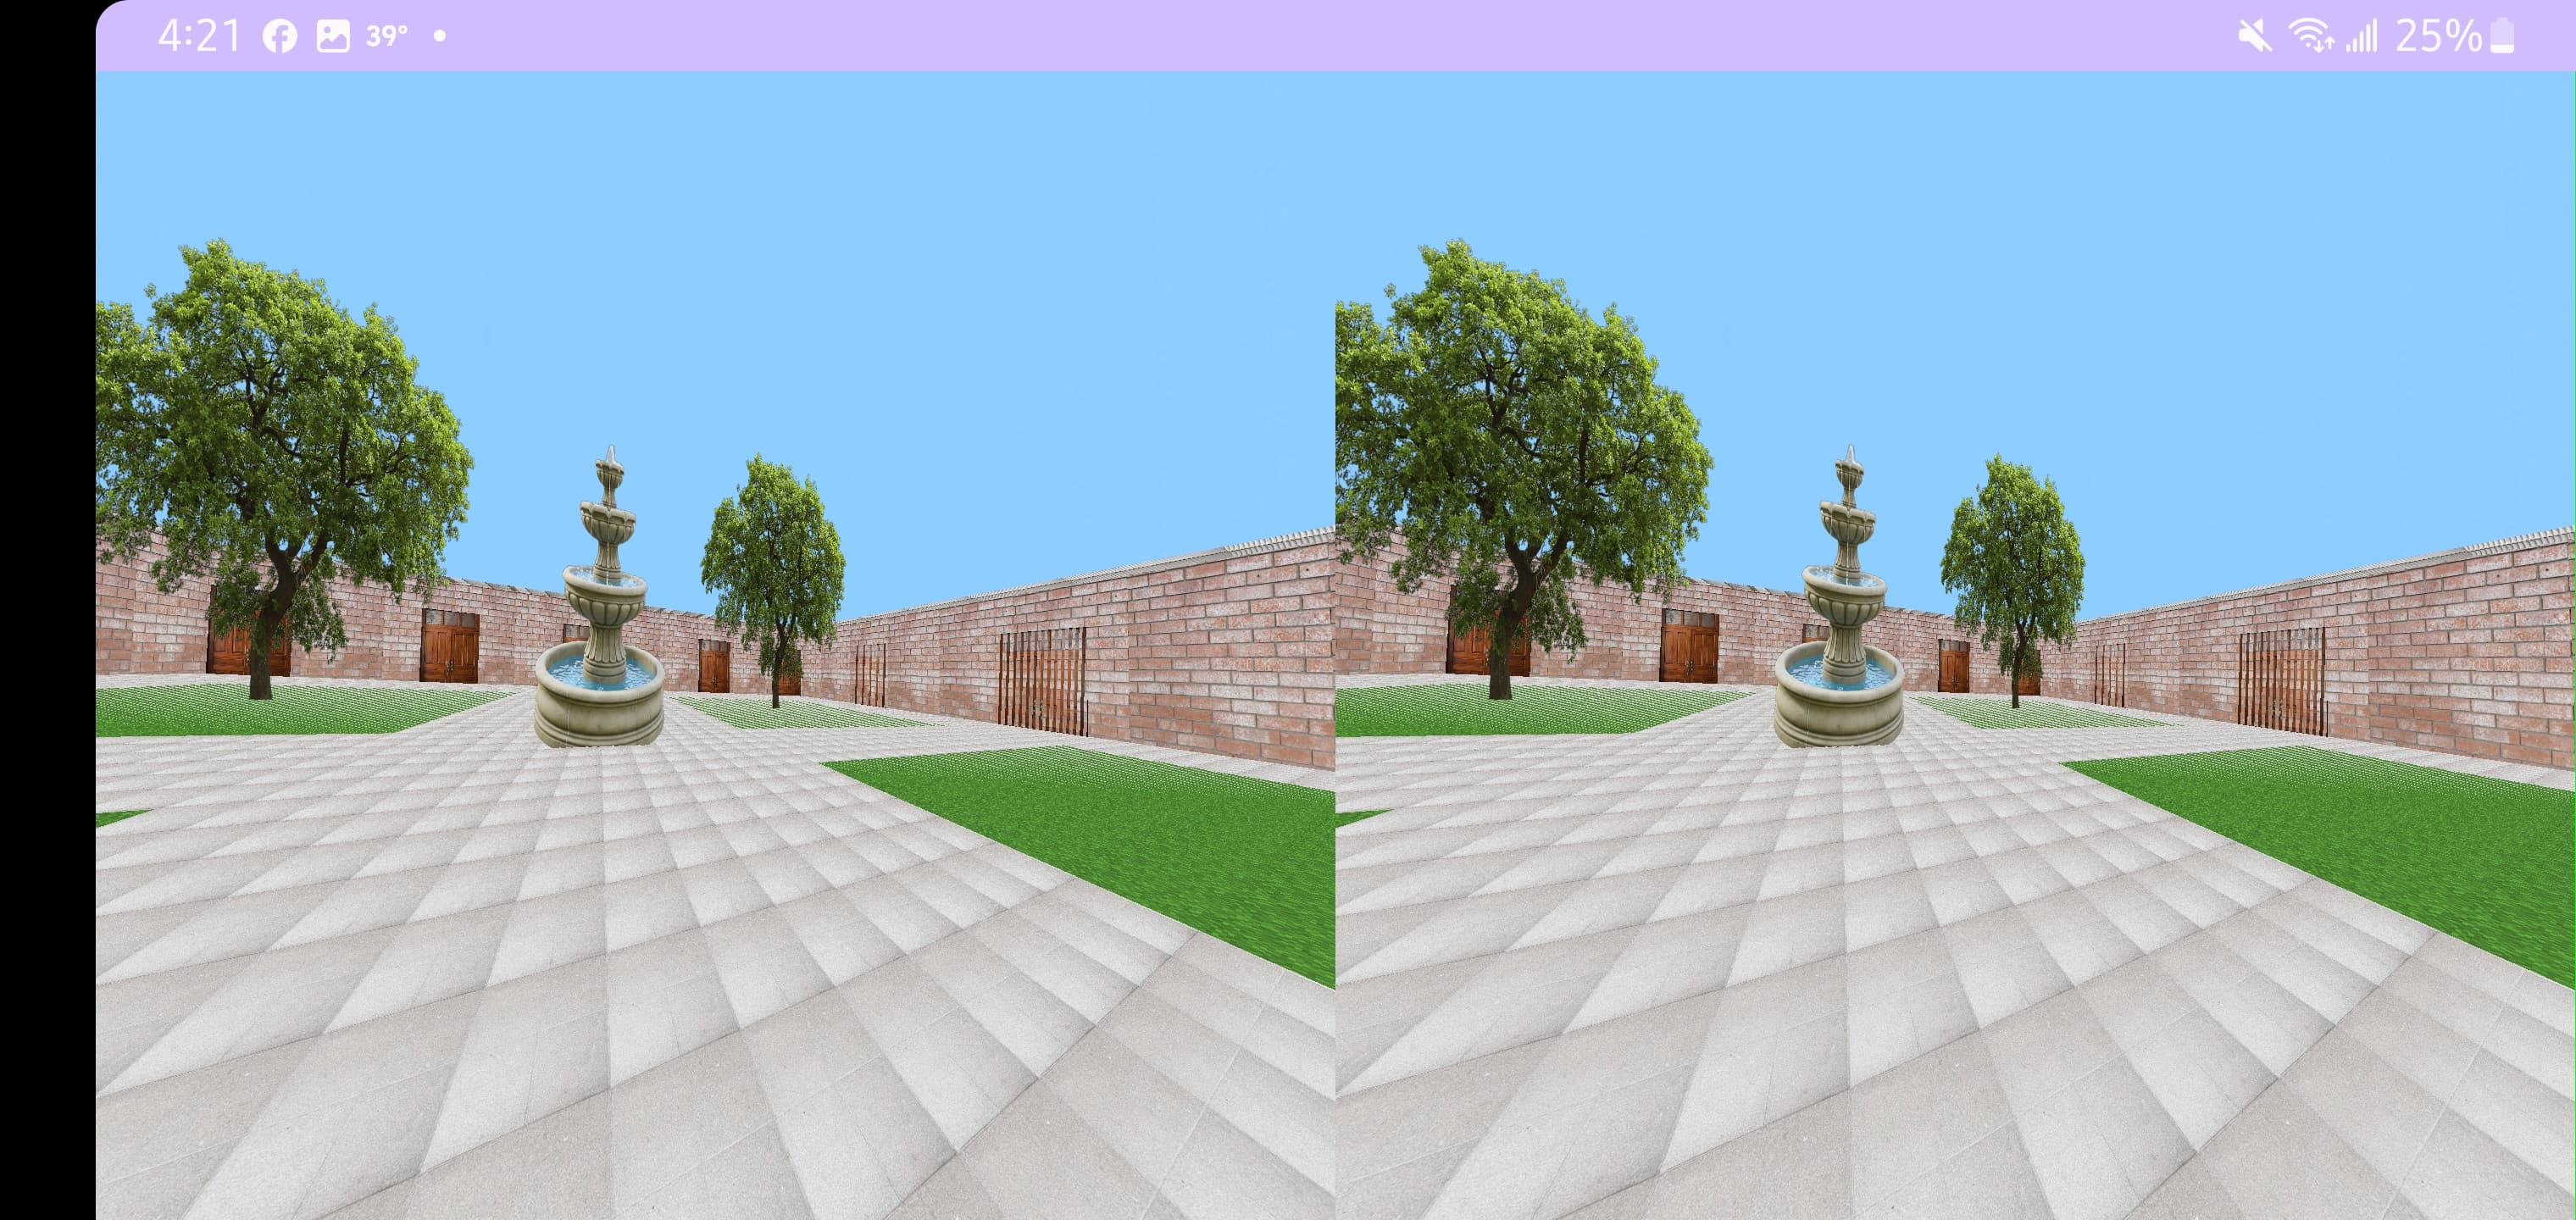
\includegraphics[width=\columnwidth]{demo_original.png}
		\caption{Versión previa a la migración. La escena se renderiza dos veces
			con la misma cámara, sin separación interpupilar ni distorsión de barril,
			produciendo un ``pseudo-estéreo'' que no aprovecha un visor real.}
		\label{fig:original}
	\end{figure}
	
	Tras la migración, la aplicación arranca en una pantalla de bienvenida que
	presenta el mapeo de controles del mando físico e identifica a los
	desarrolladores del equipo. La Figura~\ref{fig:vrmenu} muestra esta pantalla
	ya renderizada en modo Cardboard: la imagen se divide en dos vistas
	independientes, una por ojo, cada una con la deformación de barril necesaria
	para compensar la óptica de las lentes del visor.
	
	\begin{figure}[htbp]
		\centering
		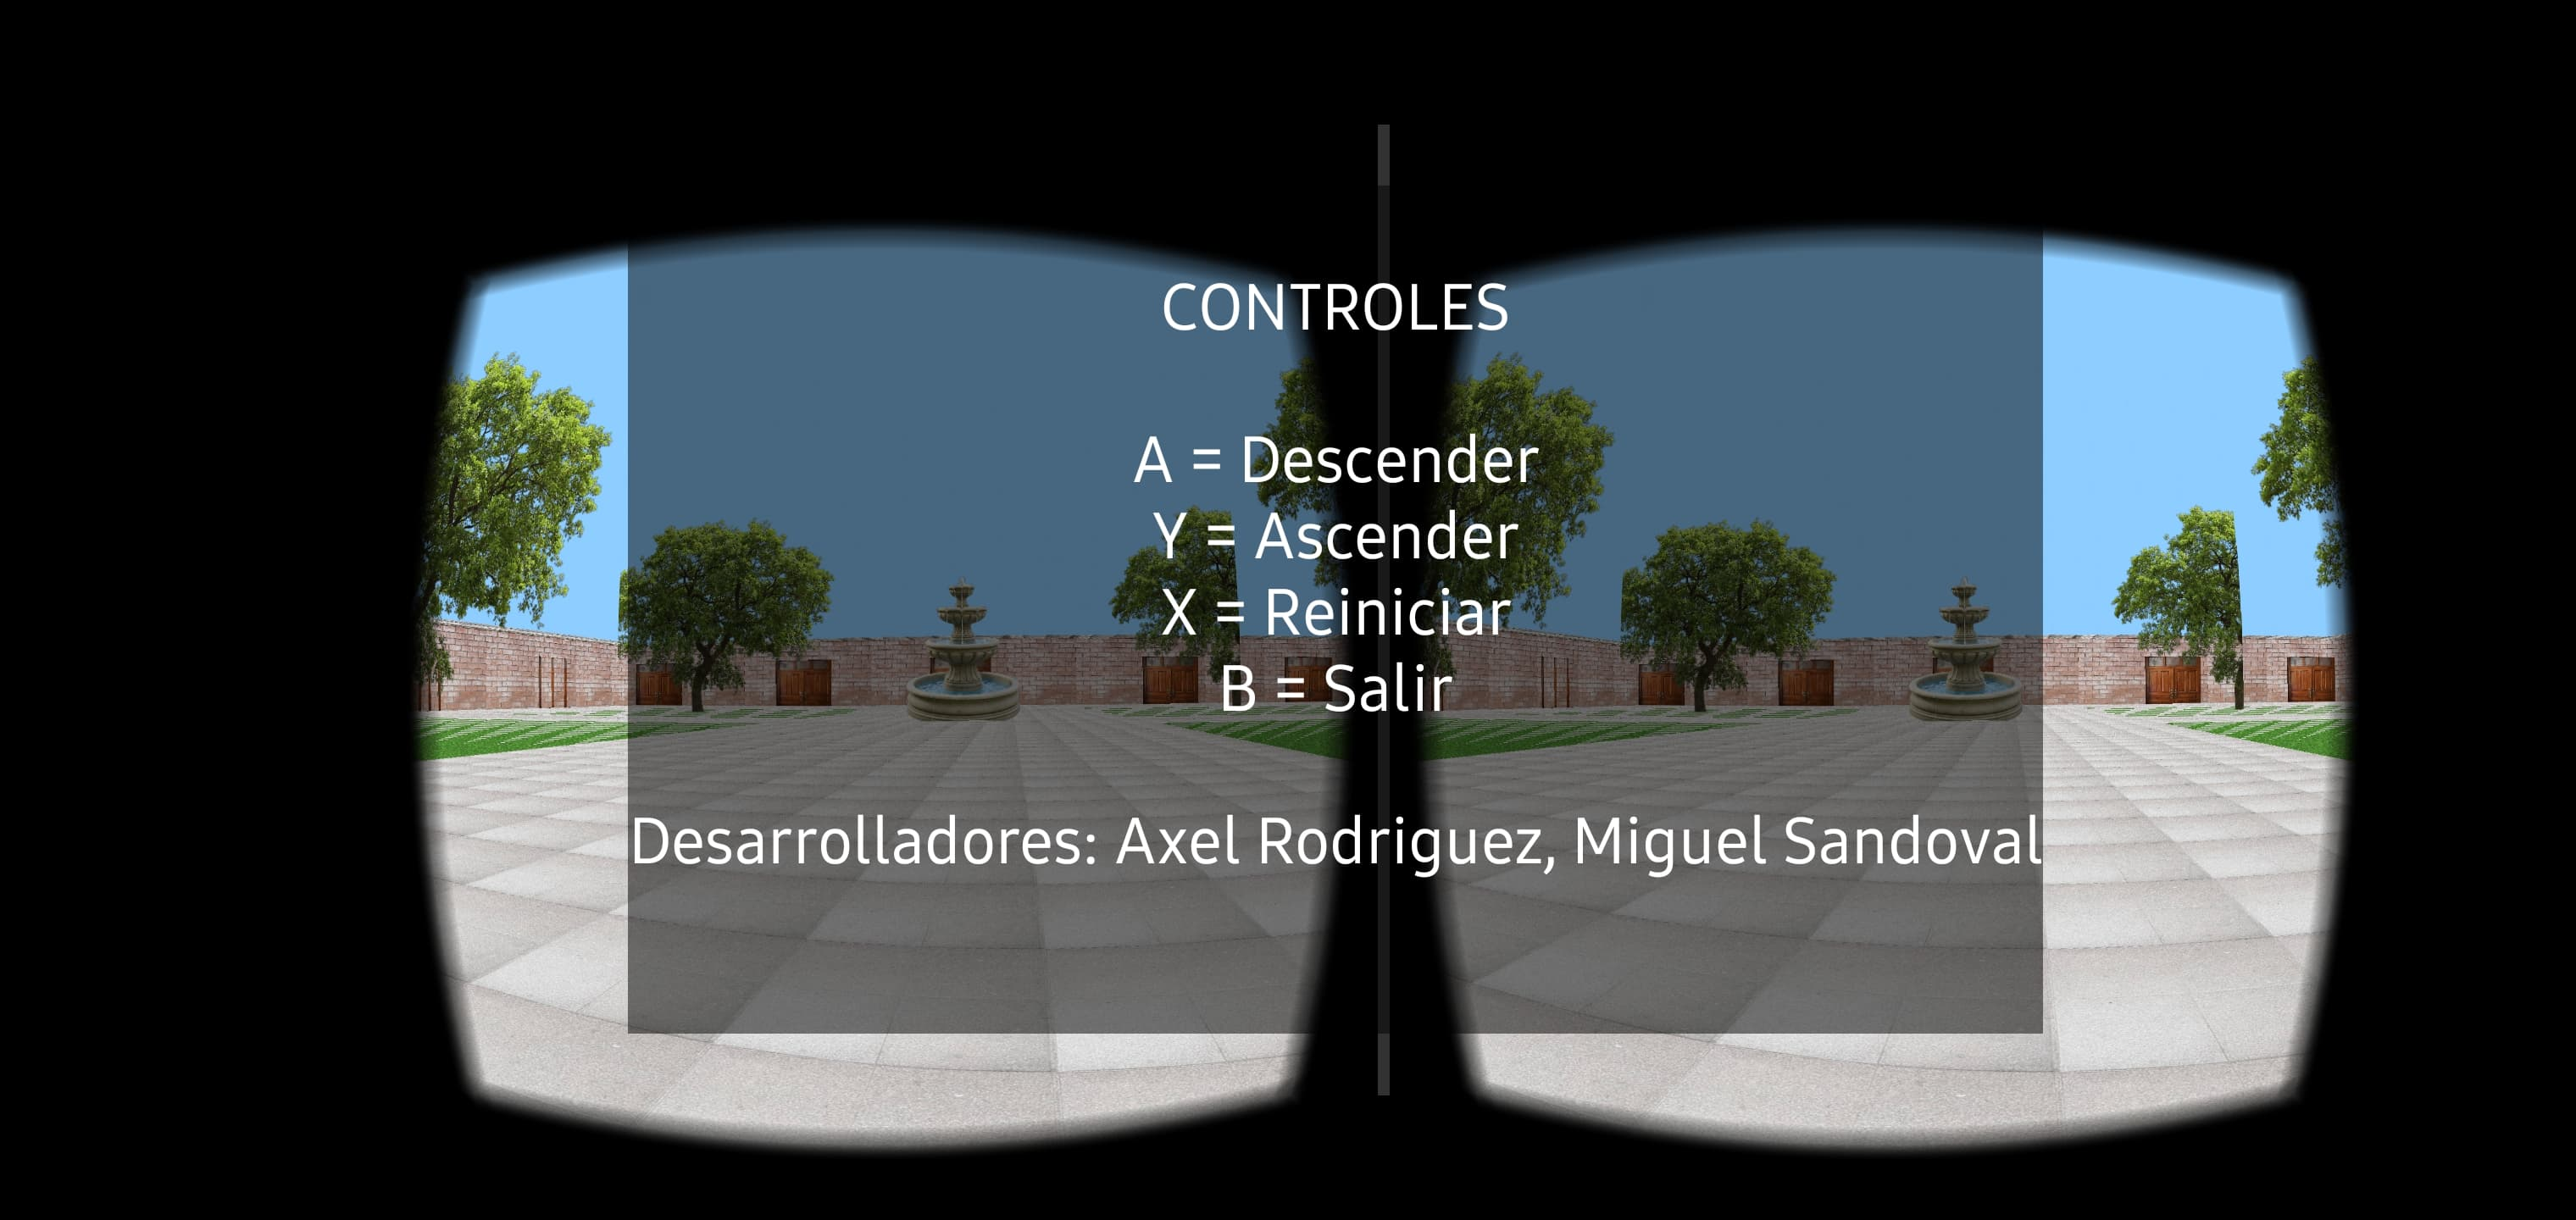
\includegraphics[width=\columnwidth]{vr_menu.png}
		\caption{Pantalla de bienvenida y controles en modo VR. Cada ojo recibe
			una vista propia con distorsión de barril; el menú superpone el mapeo de
			botones (A=Descender, Y=Ascender, X=Reiniciar, B=Salir).}
		\label{fig:vrmenu}
	\end{figure}
	
	Durante el recorrido, el usuario navega por el patio, los jardines y la
	fachada del edificio orientando la cabeza (seguimiento por los sensores del
	teléfono) y desplazándose con el mando. La Figura~\ref{fig:vrrecorrido}
	captura un momento del recorrido por la plaza central: se aprecia la
	separación interpupilar real entre ambas vistas y la curvatura característica
	de la corrección de lente, elementos ausentes en la versión original.
	
	\begin{figure}[htbp]
		\centering
		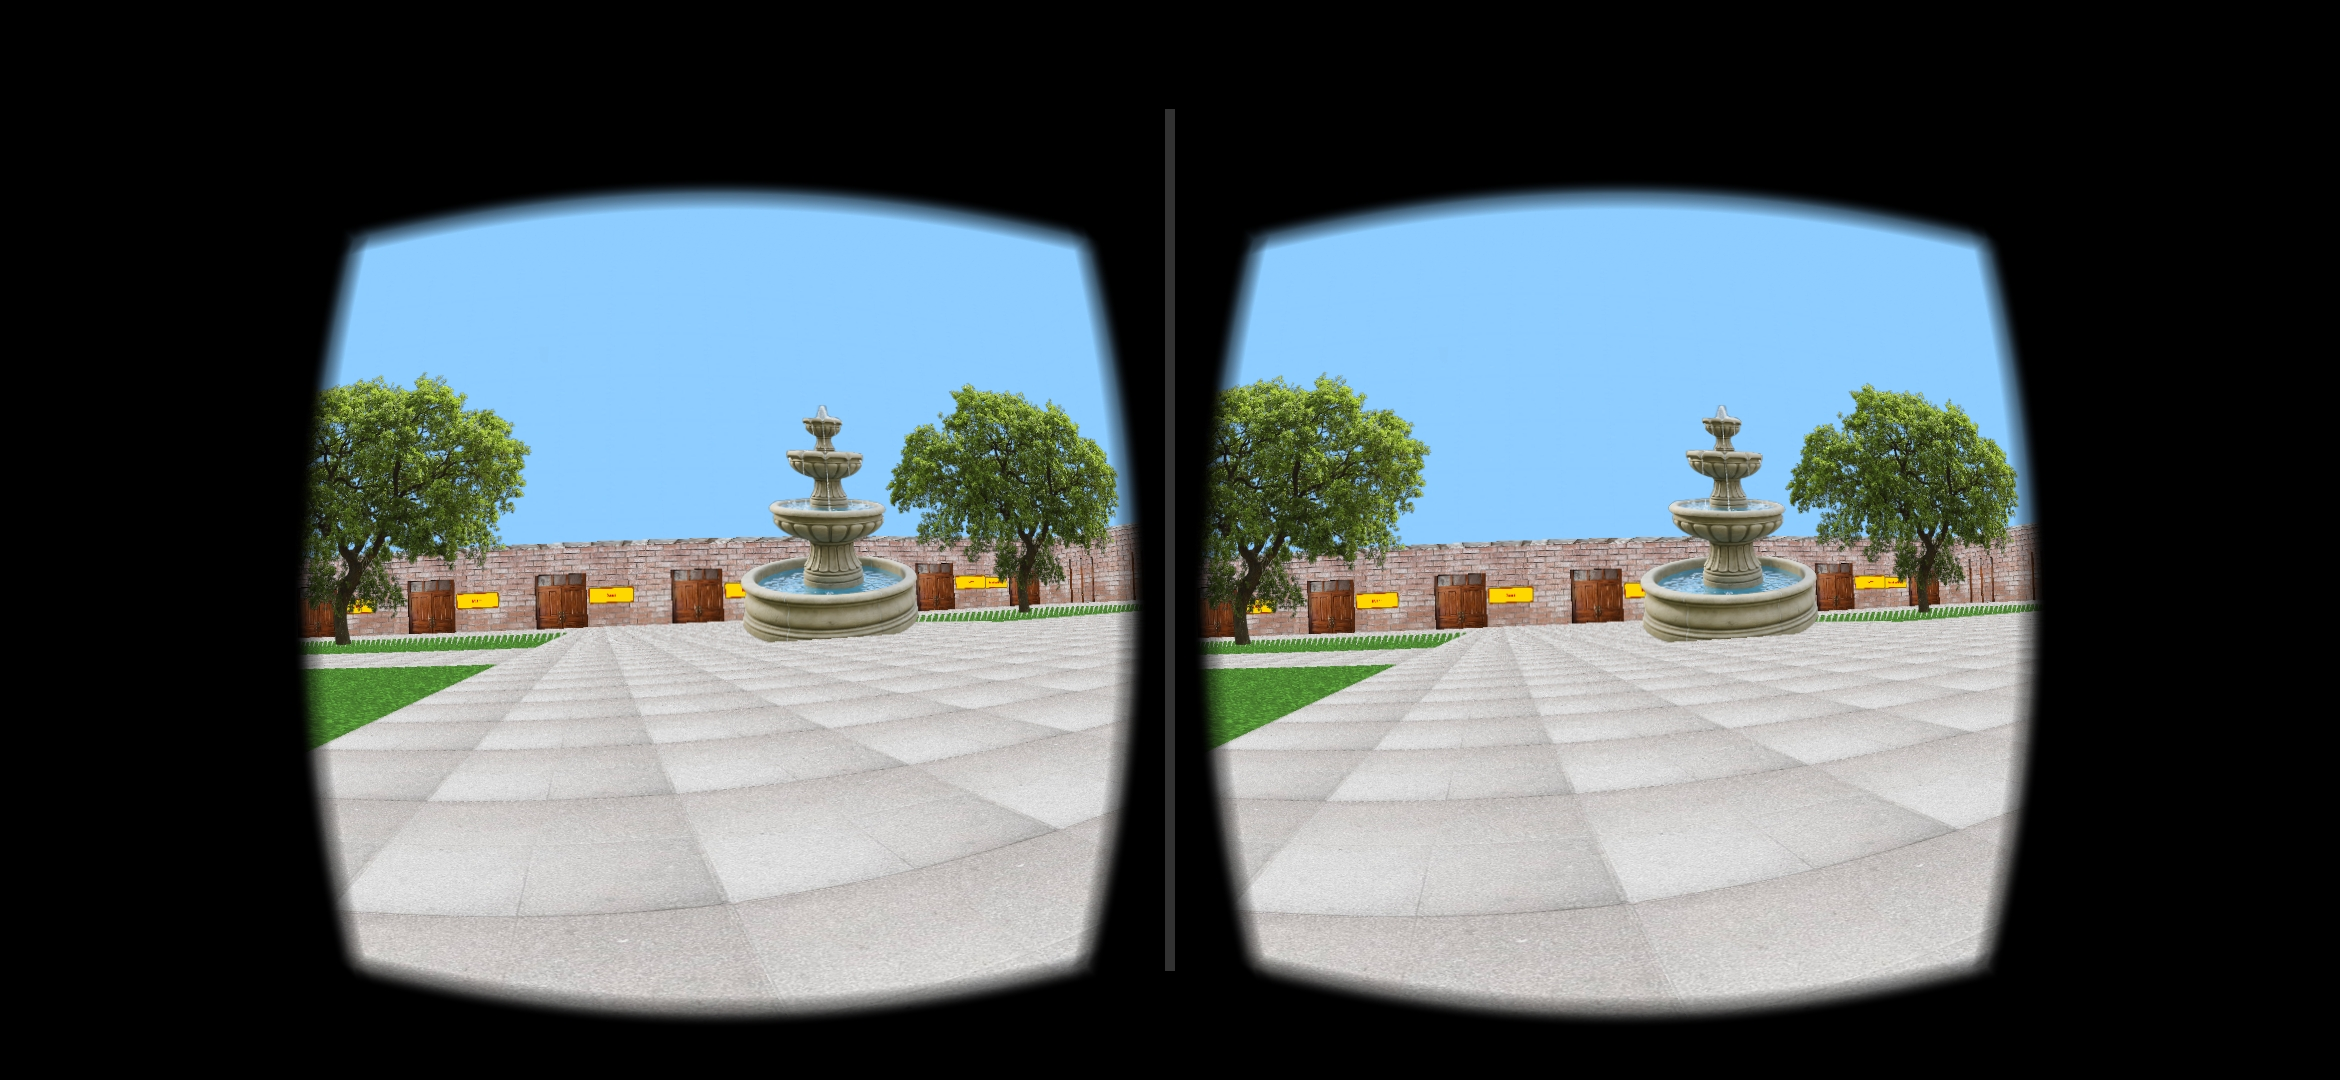
\includegraphics[width=\columnwidth]{vr_recorrido.png}
		\caption{Recorrido inmersivo por la plaza central del modelo en modo VR.
			Ambas vistas presentan separación interpupilar y distorsión de barril,
			listas para un visor Cardboard.}
		\label{fig:vrrecorrido}
	\end{figure}
	
	En conjunto, los resultados verificables de la migración son:
	
	\begin{itemize}
		\item Renderizado estéreo real (una cámara por ojo) con separación
		interpupilar, frente a la vista duplicada de la versión original.
		\item Corrección de distorsión de lente (barril) aplicada por ojo,
		requisito indispensable para un visor Cardboard.
		\item Navegación por orientación de la cabeza mediante los sensores del
		dispositivo, además del control con mando físico ya existente.
		\item Reutilización íntegra de la geometría y las texturas del proyecto
		original, sin pérdida de contenido visual en la escena.
	\end{itemize}
	
	Como parte de las correcciones solicitadas por el instructor, se verificó y corrigió la cantidad de puertas que hay en la demo, añadiendo sus respectivos nombres de acuerdo a la sala que corresponde. La Figura~\ref{fig:nombres_puertas} ilustra este resultado, mostrando los accesos a las salas de ``Dirección'' y ``Fotografía, Oratoria, Composición Literaria''.
	
	\begin{figure}[htbp]
		\centering
		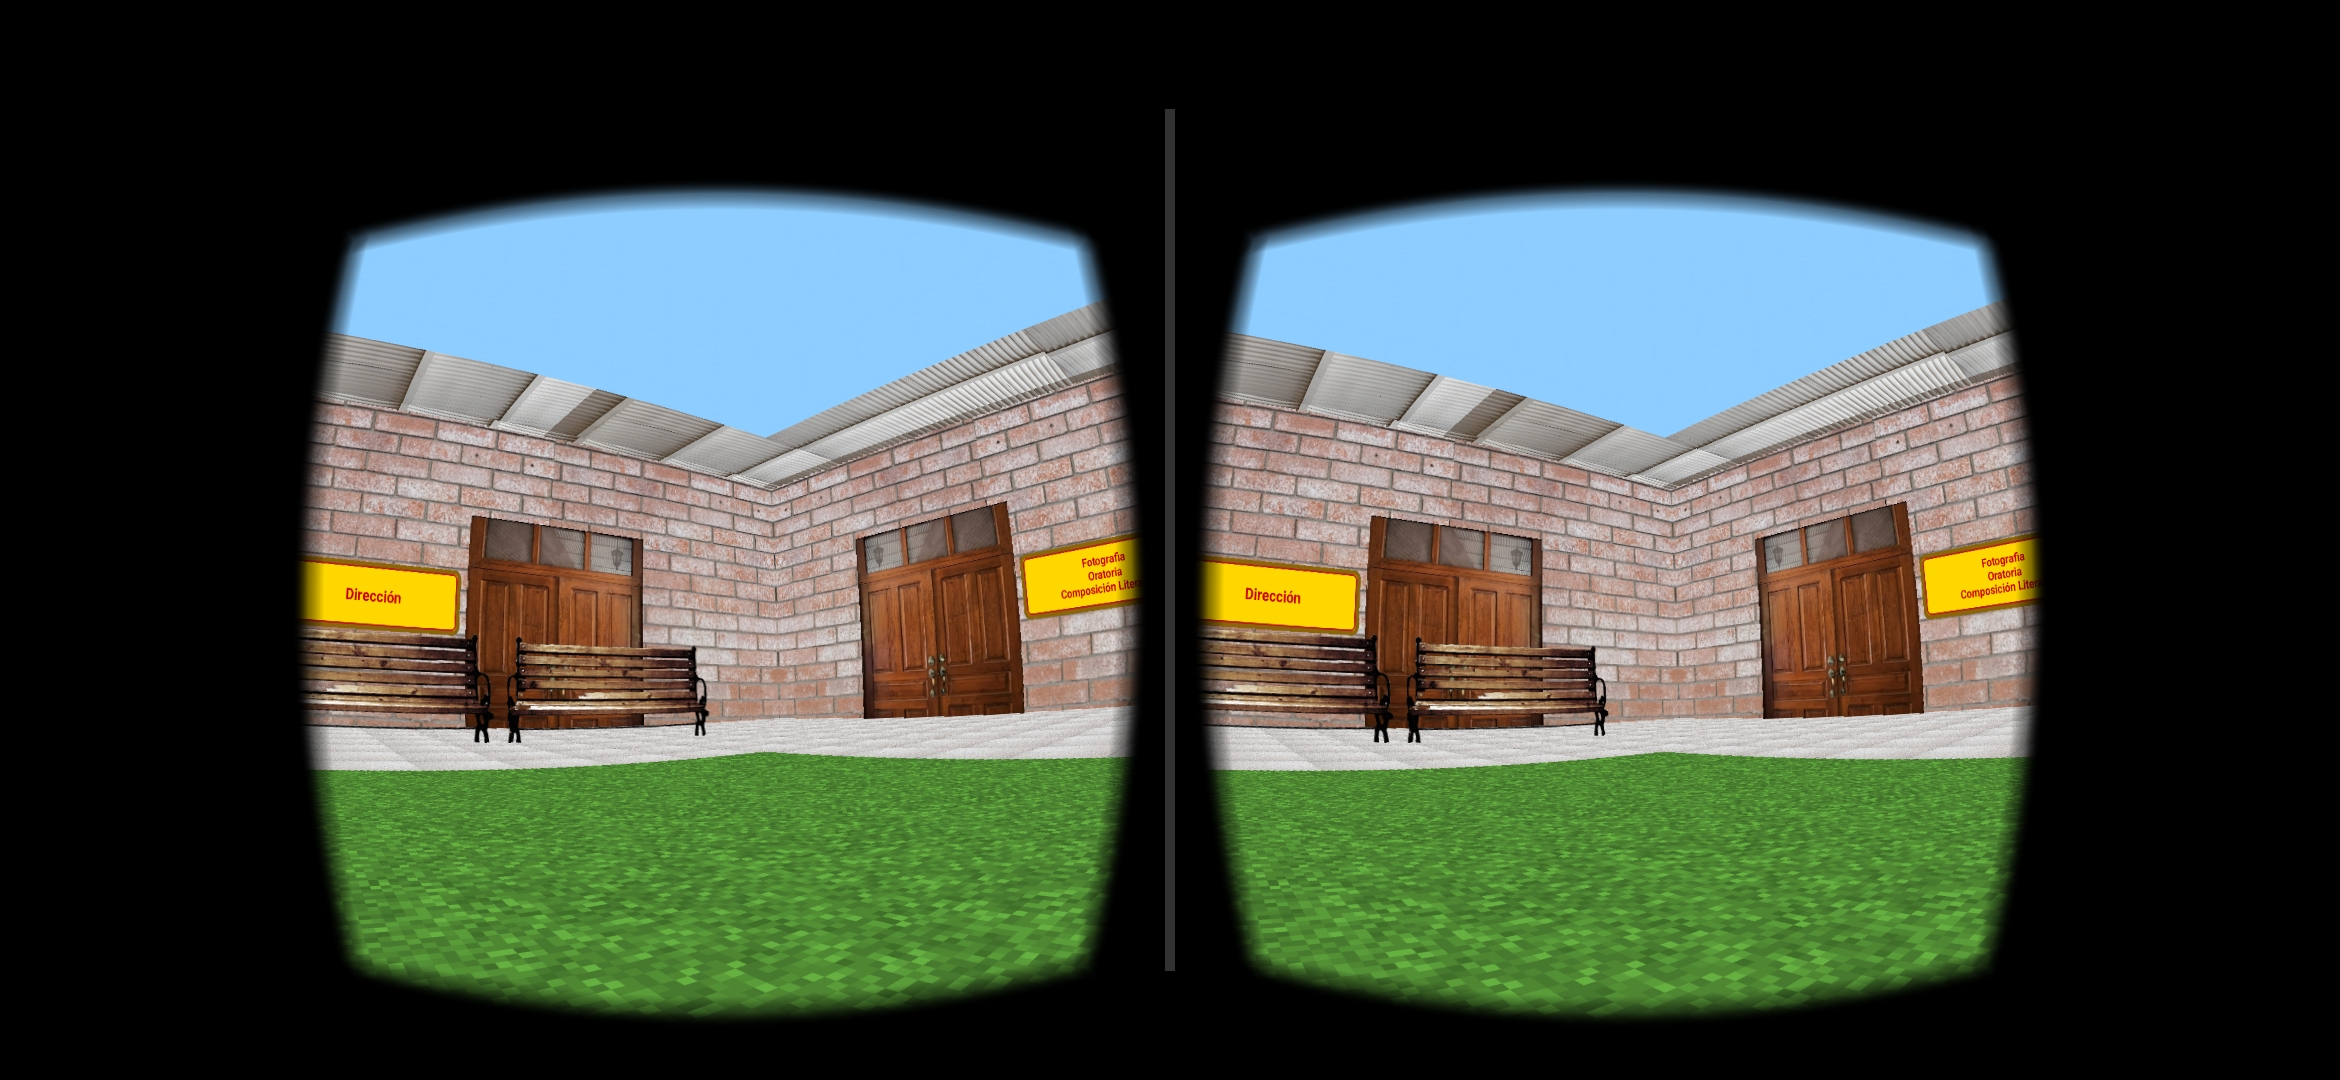
\includegraphics[width=\columnwidth]{correccion.png}
		\caption{Vista inmersiva evidenciando la corrección en la cantidad de puertas y la asignación de sus respectivos nombres de acuerdo a la sala.}
		\label{fig:nombres_puertas}
	\end{figure}
	
	\section{Conclusión}
	La migración de \textit{Casa del Arte} demuestra que es posible transformar un recorrido 3D convencional en una experiencia de realidad virtual genuina~\cite{slater1997five} sin reconstruir el contenido tridimensional ya existente: bastó con remplazar la capa de renderizado y de captura de movimiento --de una \texttt{Activity} con \texttt{GLSurfaceView} y un mecanismo manual de doble dibujado por mitades de pantalla, a una \texttt{CardboardActivity} con \texttt{CardboardView.StereoRenderer}-- para pasar de una simulación superficial de estereoscopía, sin separación interpupilar ni seguimiento de cabeza, a una experiencia con seguimiento real de la orientación del usuario, corrección de distorsión de lente y retroalimentación háptica, todo ello provisto por el Google Cardboard SDK. La totalidad de la geometría procedural del recinto (prismas y planos con textura que conforman paredes, ventanas, puertas, techos, jardines, banquetas y portón) se conservó intacta, lo que confirma que la separación original entre la lógica de construcción de la escena y la lógica de renderizado facilitó considerablemente esta migración.
	
	No obstante, la revisión del código evidenció áreas de mejora relevantes para futuras iteraciones del proyecto: eliminar el código muerto detectado en \texttt{TextureHelper} (heredado sin cambios desde la versión original), depurar los recursos de imagen sin uso, resolver por completo los límites de desplazamiento en los ejes X y Z --pendiente señalado por el propio equipo desde antes de la migración--, y reorganizar el proyecto conforme a la estructura estándar de Android Studio para facilitar su compilación, mantenimiento y colaboración entre los integrantes del equipo.
	
	\addcontentsline{toc}{section}{Referencias}
	\printbibliography
	
\end{document}